As the modeling of the CMS detector and underlying physics processes are imperfect, scale factors and corrections are applied to Monte Carlo events and in some cases, the embedded samples, to improve agreement with measurements in data. For the standard reconstruction physics objects in this work, central recommendations provided by dedicated physics object groups (POGs) in CMS are used.

Uncertainties in scale factors and corrections are also sources of systematic errors in the analysis, detailed in Chapter \ref{chapter:ch-11:systematic-uncertainties}. Systematic uncertainties in the tau, muon, and electron energy scales can shift the $p_{T}$ of the leptons up or down, causing a migration of number of events that pass the offline $p_{T}$ thresholds described in the previous section.

\section{Tau energy scale}

An energy scale is applied to the transverse momentum $p_{T}$ and mass of the hadronic tau $\tau_{h}$ in the $\mu\tau_{h}$ and $e\tau_{h}$ channels, to correct for a deviation of the average reconstructed $\tau_{h}$ energy from the generator-level energy of the visible $\tau_{h}$ decay products. These correction factors are derived centrally \cite{CMS-TAU-16-003}, by fitting to events in $e\tau_{h}$ and $\mu\tau_{h}$ final states in $Z/\gamma^*$ events separately for the $h^\pm$, $h^\pm \pi^0$, and $h^\pm h^\mp h^\pm$ decays. The values used are shown in Table \ref{table:tau-ES}.

When applying the energy scale to the $\tau_{h}$, the 4-momentum of the missing transverse energy (MET) is adjusted such that the total 4-momenta of the $\tau_{h}$ and the MET remains unchanged \cite{twiki_TAU_POG_tauidrecommendationforrun2}.

\begin{table}[ht]
    \centering
    \begin{tabular}{|c|c|c|c|c|}
    \hline
    \multicolumn{5}{|c|}{Tau energy scale factor}                                   \\ \hline
    \hline
    Decay mode      & 2018              & 2017              & 2016 pre-VFP      & 2016 post-VFP     \\ \hline
    0               & 0.991 $\pm$ 0.008 & 0.986 $\pm$ 0.009 & 0.987 $\pm$ 0.01  & 0.993 $\pm$ 0.009 \\
    1               & 1.004 $\pm$ 0.006 & 0.999 $\pm$ 0.006 & 0.998 $\pm$ 0.006 & 0.991 $\pm$ 0.007 \\
    10              & 0.998 $\pm$ 0.007 & 0.999 $\pm$ 0.007 & 0.984 $\pm$ 0.008 & 1.001 $\pm$ 0.007 \\
    11              & 1.004 $\pm$ 0.009 & 0.996 $\pm$ 0.01  & 0.999 $\pm$ 0.011 & 0.997 $\pm$ 0.016 \\ \hline
    \end{tabular}
    \caption{Energy scales applied to genuine hadronic tau decays $\tau_{h}$ by data-taking year/era and decay mode, along with systematic errors.}
    \label{table:tau-ES}
\end{table}

\section{Muon energy scale}
An energy scale is applied to the $p_{T}$ and mass of genuine muons from $\tau$ decays in the $e\mu$ and $\mu\tau_{h}$ channels \cite{twiki_MUON_POG_recommendation}. The applied values are the same for MC and embedded samples and are shown in Table \ref{table:muon-ES}. Following the SM $H \rightarrow \tau\tau$ analysis, Rochester corrections are not applied, and instead prescriptions from \cite{twiki_MUO_simplified_ES} are followed.


\begin{table}[ht]
    \centering
    \begin{tabular}{|c|c|}
    \hline
    \multicolumn{2}{|c|}{Muon energy scale factor}      \\ \hline
    \hline
    Eta range                & Value for all years \\ \hline
    $|\eta| \in [0.0, 1.2)$  & 1.0 $\pm$ 0.004 \\
    $|\eta| \in [1.2, 2.1)$  & 1.0 $\pm$ 0.009 \\
    $|\eta| \in [2.1, 2.4)$  & 1.0 $\pm$ 0.027 \\
    \hline
    \end{tabular}
    \caption[Energy scales and systematic errors applied to genuine muons.]{Energy scales and systematic errors applied to genuine muons. The values are the same for MC and embedded for all years \cite{twiki_HiggsToTauTauWorkingLegacyRun2} \cite{twiki_MUO_simplified_ES}.}
    \label{table:muon-ES}
\end{table}


\section{Electron energy scale}
Corrections to the electron energy scale are applied to genuine $e$ from $\tau$ decays, and are binned in two dimensions by electron $p_{T}$ and $\eta$ for barrel vs. endcap \cite{twiki_Electron_POG_recommendation}. The scale factors are binned in $p_{T}$ and $\eta$ for MC samples: e.g. values for 2018 are shown in Fig. \ref{fig:egamma-POG-UL-egamma-scale-factors} from \cite{twiki_Electron_UL_2016_2017_2018}. For embedded samples the electron energy scale is taken as only binned in $\eta$ (Table \ref{table:ele-ES-embedded}).

% https://twiki.cern.ch/twiki/pub/CMS/EgammaUL2016To2018/egammaEffi.txt_Ele_wp90noiso_egammaPlots.pdf
\begin{figure}[h]
    \centering
    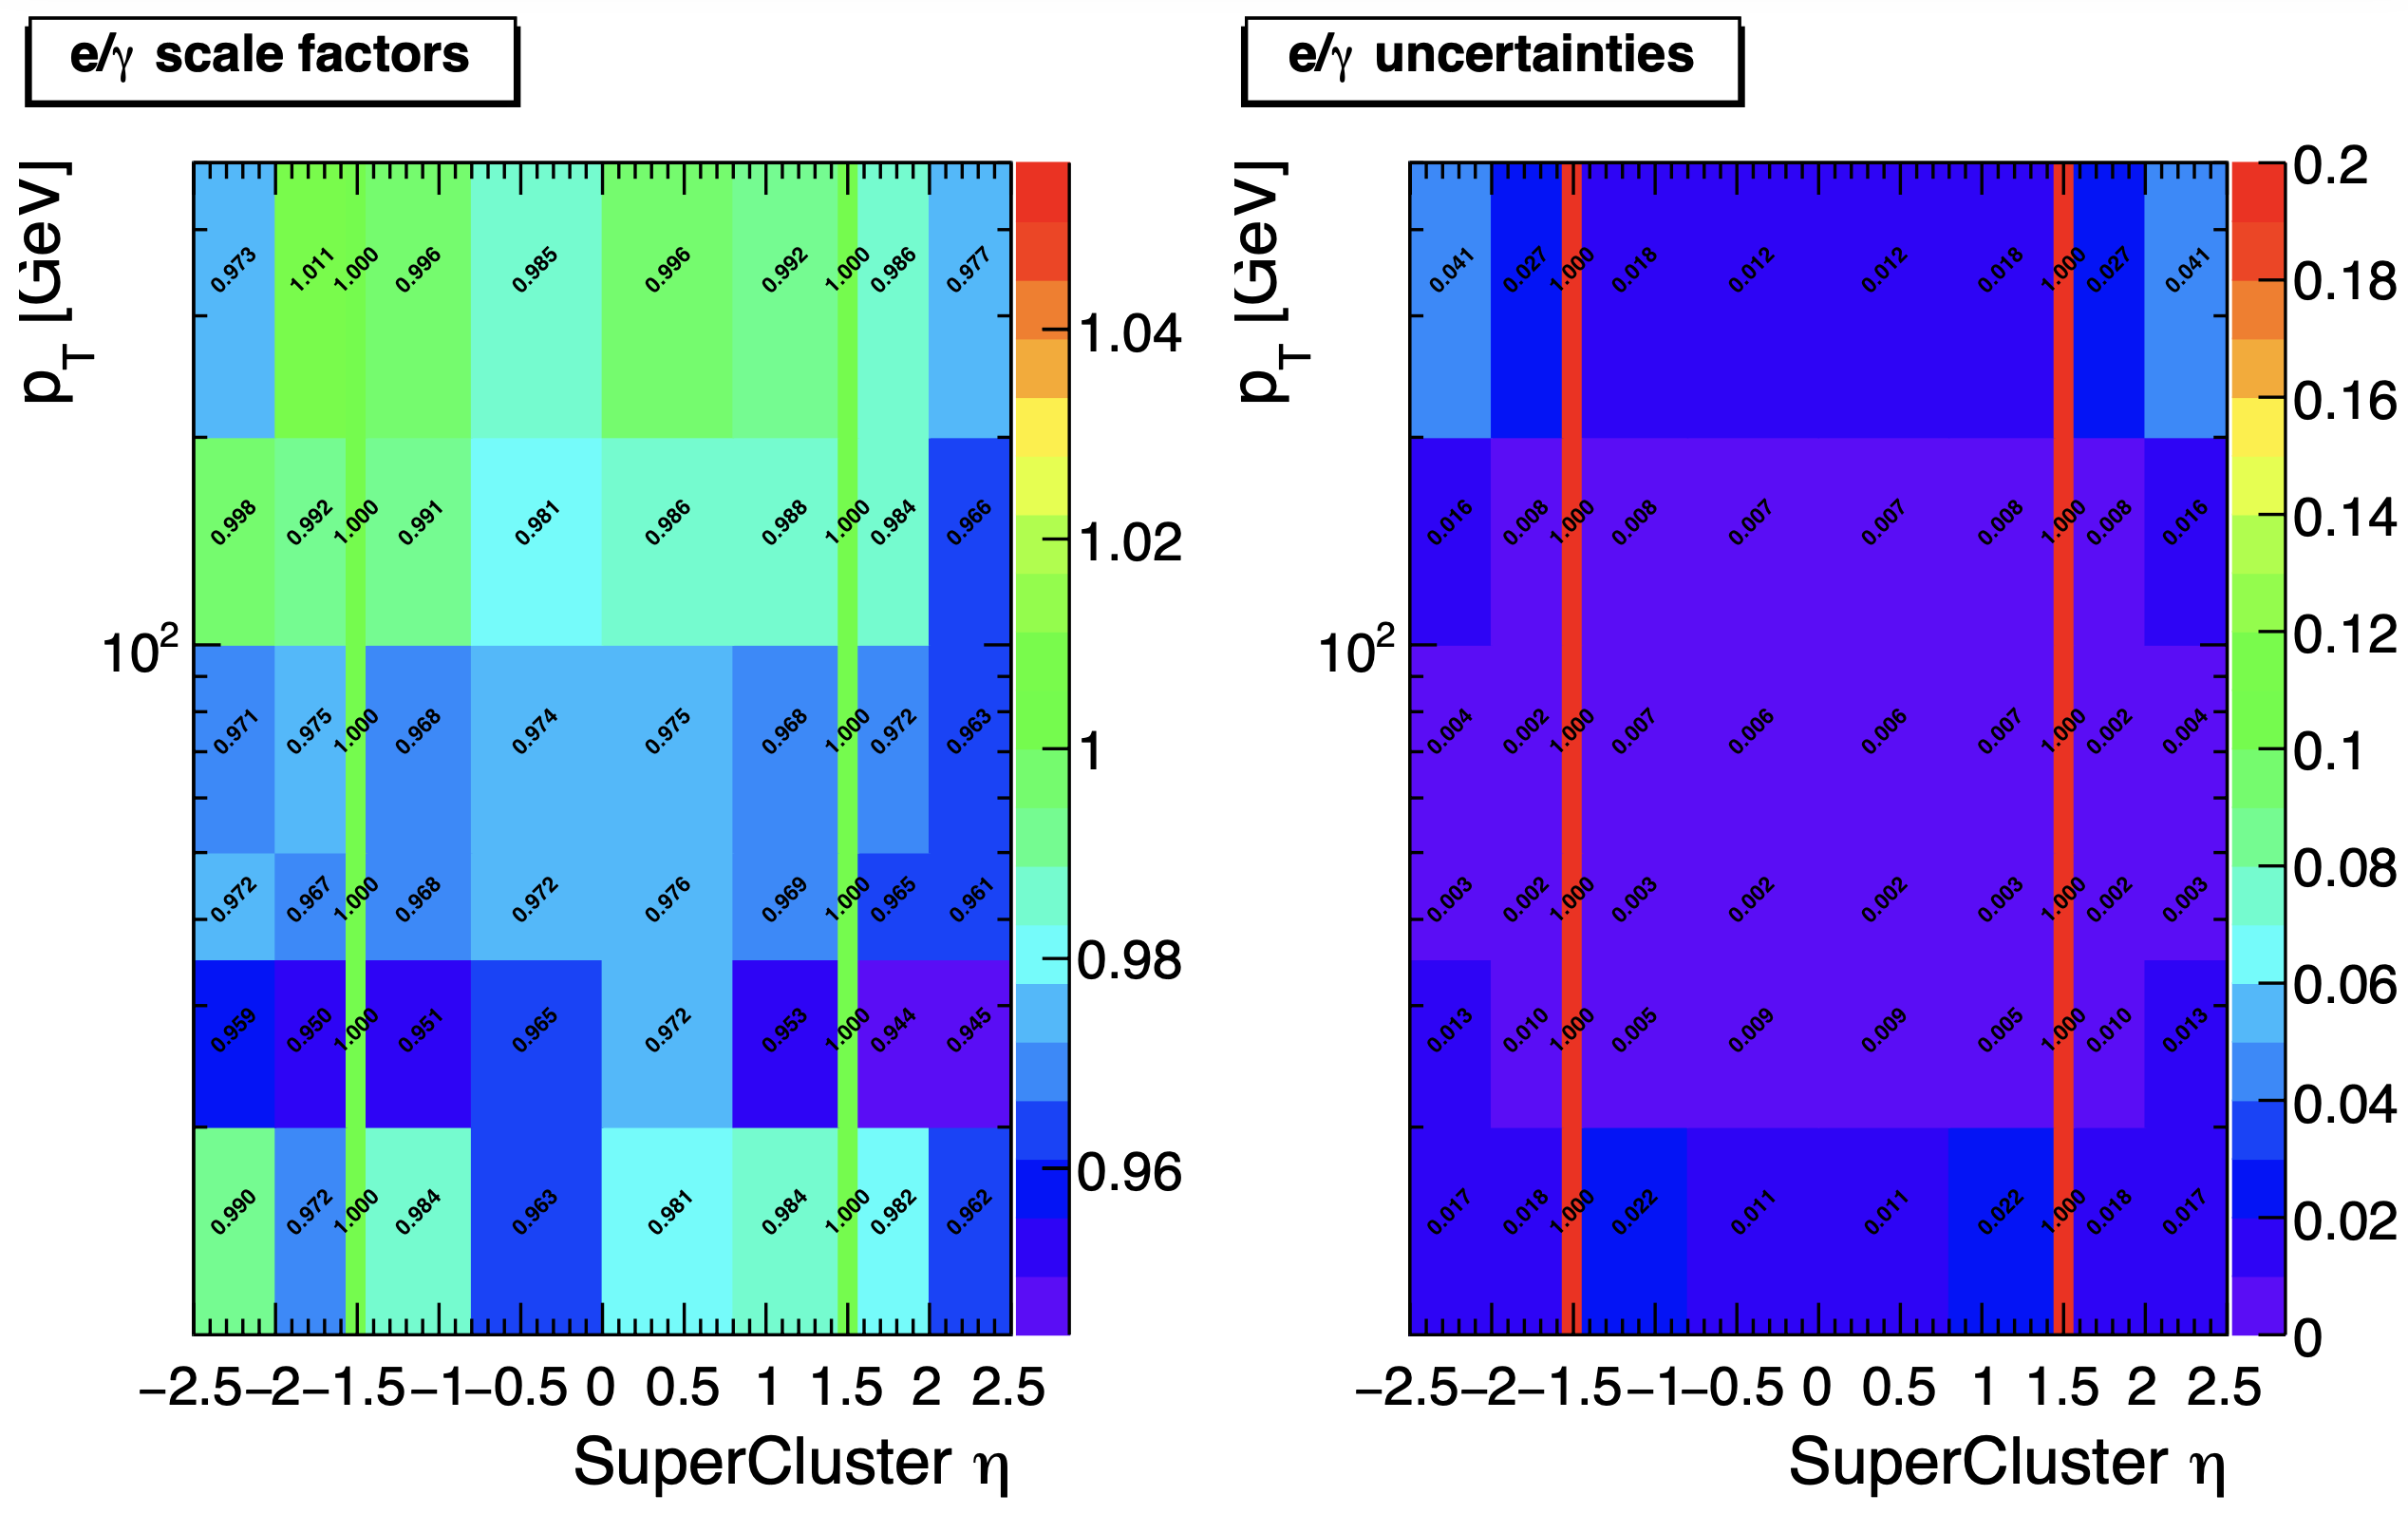
\includegraphics[width=15cm]{figures/ch-8-scale-factors-and-corrections/egamma-POG-UL-egamma-scale-factors.png}
    \caption[Electron/photon energy scale factors and uncertainties for 2018.]{Electron/photon energy scale factors (\textit{left}) and corresponding uncertainties (\textit{right}) binned in the electron $\eta$ and $p_{T}$, for the data-taking year 2018 \cite{twiki_Electron_UL_2016_2017_2018}.} 
    \label{fig:egamma-POG-UL-egamma-scale-factors}
\end{figure}


\begin{table}[h]
    \centering
    \begin{tabular}{|c|c|c|c|}
    \hline
    \multicolumn{4}{|c|}{Electron energy scale factor for embedded samples}                                   \\ \hline
    \hline
    Eta range                   & 2018               & 2017               & 2016     \\ \hline
    $|\eta| \in [0.0, 1.479)$   & 0.973 $\pm$ 0.005  & 0.986 $\pm$ 0.009  & 0.9976 $\pm$ 0.0050 \\
    $|\eta| \in [1.479, 2.4)$   & 0.980 $\pm$ 0.0125 & 0.887 $\pm$ 0.0125 & 0.993 $\pm$ 0.0125 \\ \hline
    \end{tabular}
    \caption[Energy scales and systematic errors applied to electrons in embedded samples by data-taking year/era.]{Energy scales and systematic errors applied to electrons in embedded samples, binned in the electron $\eta$, by data-taking year \cite{twiki_embedded_preUL_2016} \cite{twiki_embedded_preUL_2017} \cite{twiki_embedded_preUL_2018}.}
    \label{table:ele-ES-embedded}
\end{table}

\section{$\tau_{h}$ identification efficiency}
The $\tau_{h}$ identification efficiency can differ in data and MC \cite{twiki_TAU_POG_tauidrecommendationforrun2}. Recommended corrections are provided by the Tau POG, and we use the medium DeepTau vs. jet working point values. The identification efficiency is measured in $Z \rightarrow \tau\tau$ events in the $\mu\tau_{h}$ final state, and is binned in $p_{T}$ due to clear $p_{T}$ dependence of the DeepTau ID. 


\begin{table}[h]
    \centering
    \begin{tabular}{|c|c|c|c|c|c|c|}
    \hline
    \multicolumn{7}{|c|}{Tau ID efficiency for DeepTau Medium vs. jet WP in 2018}                                   \\ \hline
    \hline
    $p_{T}$ (GeV)  & $<20$  & $(20, 25]$ & $(25, 30]$ & $(30, 35]$ & $(35, 40]$ & $(40, 500] $   \\ \hline
    Central value  & 0      & 0.945      & 0.946      & 0.916      & 0.921      & 1.005 \\
    Up value       & 0      & 1.001      & 0.981      & 0.946      & 0.950      & 1.035 \\
    Down value     & 0      & 0.888      & 0.981      & 0.883      & 0.893      & 0.953 \\ \hline
    \end{tabular}
    \caption[Tau ID efficiency for the DeepTau vs. jet medium working point, with central, up, and down values for 2018, binned in the tau $p_{T}$.]{Tau ID efficiency for the DeepTau vs. jet medium working point, with central, up, and down values for 2018, binned in the tau $p_{T}$ \cite{twiki_TAU_POG_tauidrecommendationforrun2}.}
    \label{table:tauIDeff_deepTau_vs_jet_medium_WP}
\end{table}


\section{Electrons and muons faking $\tau_{h}$: energy scales}

Energy scales for electrons misidentified as hadronic tau decays ($e$ faking $\tau_{h}$) are provided by the Tau POG, and were measured in the $e\tau_{h}$ channel with the visible invariant mass of the electron and hadronic tau system \cite{twiki_HiggsToTauTauWorkingLegacyRun2}. This energy scale is applied for $\tau_{h}$ with $p_{T} > 20$ GeV regardless of which DeepTau vs. electron working point was used. Values for 2018 are shown in Table \ref{table:electron-faking-tauh-FES-2018}.

% root -l TauFES_eta-dm_DeepTau2017v2p1VSe_2018ReReco.root 
\begin{table}[h]
    \centering
    \begin{tabular}{|c|c|}
    \hline
    \multicolumn{2}{|c|}{Electrons faking $\tau_{h}$ energy scale factor in 2018}      \\ \hline
    \hline
    Reconstructed decay mode of the fake $\tau_{h}$  & Central value and (up, down) shifts \\ \hline
    0   & 1.01362 (+0.00474, -0.00904) \\
    1   & 1.01945 (+0.01598, -0.01226) \\
    10  & 0.96903 (+0.0125, -0.03404) \\
    11 & 0.985 (+0.04309, -0.05499) \\ \hline
    \end{tabular}
    \caption[Energy scales and up/down systematic uncertainties applied to electrons misidentified as hadronic taus.]{Energy scales and up/down systematic uncertainties applied to electrons misidentified as hadronic taus \cite{twiki_HiggsToTauTauWorkingLegacyRun2} for 2018, binned in decay mode of the fake $\tau_{h}$.}
    \label{table:electron-faking-tauh-FES-2018}
\end{table}

No nominal energy scale is applied for muons mis-reconstructed as $\tau_{h}$, and the uncertainty is treated as $\pm$ 1\% and uncorrelated in the reconstructed decay mode \cite{twiki_HiggsToTauTauWorkingLegacyRun2}. 

\section{Electrons and muons faking $\tau_{h}$: misidentification efficiencies}
Corrections on identification efficiencies are applied to genuine electrons and muons misidentified as $\tau$ to account for differences in data and MC.

The specific values depend on the vs. electron and vs. muon discriminator working points used. 
For misidentified $\mu \rightarrow \tau_{h}$, the scale factors are split into different $|\eta|$ regions, determined by the CMS muon and tracker detector geometries, as shown in Table \ref{table:tauIDeff_deepTau_vs_muon} for 2018 \cite{twiki_TAU_POG_tauidrecommendationforrun2}.


\begin{table}[h]
    \centering
    \begin{tabular}{|c|c|c|}
    \hline
    \multicolumn{3}{|c|}{Tau ID efficiency for DeepTau vs. muon WPs in 2018}                                   \\ \hline
    \hline
    $|\eta|$  & Tight working point & VLoose working point \\ \hline
    (0.0, 0.2)     & 0.767 $\pm$ 0.127  & 0.954 $\pm$ 0.069  \\ \hline 
    (0.2, 0.6)     & 1.255 $\pm$ 0.258  & 1.009 $\pm$ 0.098  \\ \hline 
    (0.6, 1.0)     & 0.902 $\pm$ 0.203  & 1.029 $\pm$ 0.075 \\ \hline 
    (1.0, 1.45)    & 0.833 $\pm$ 0.415  & 0.928 $\pm$ 0.145\\ \hline
    (1.45, 2.0)    & 4.436 $\pm$ 0.814   & 5.000 $\pm$ 0.377 \\ \hline
    (2.0, 2.53)    & 1.000 $\pm$ 0.000         & 1.000 $\pm$ 0.000\\ \hline
    \end{tabular}
    \caption[Tau mis-identification efficiency for the DeepTau Tight and Very Loose (VLoose) working points vs. muons in 2018.]{Tau mis-identification efficiency for the DeepTau Tight and Very Loose (VLoose) working points vs. muons in 2018, binned in the muon $|\eta|$ \cite{twiki_TAU_POG_tauidrecommendationforrun2}.}
    \label{table:tauIDeff_deepTau_vs_muon}
\end{table}

For misidentified $e \rightarrow \tau_{h}$, the scale factors are split into barrel and endcap regions, dictated by the ECAL detector geometry, as shown in Table \ref{table:tauIDeff_deepTau_vs_electron} for 2018.

% root -l /Users/stephaniekwan/Dropbox/Princeton_G6/TauIDSFs/data/TauID_SF_eta_DeepTau2017v2p1VSe_2018ReReco.root 
\begin{table}[h]
    \centering
    \begin{tabular}{|c|c|c|}
    \hline
    \multicolumn{3}{|c|}{Tau ID efficiency for DeepTau vs. electron WPs in 2018}                                   \\ \hline
    \hline
    $|\eta|$  & Tight working point & VLoose working point \\ \hline
    (0.0, 0.73)     & 1.47 $\pm$ 0.27  & 0.95 $\pm$ 0.07  \\ \hline 
    (0.73, 1.509)   & 1.509 $\pm$ 0.0  & 1.00 $\pm$ 0.0  \\ \hline 
    (1.509, 1.929)  & 1.929 $\pm$ 0.2  & 0.86 $\pm$ 0.1 \\ \hline 
    (1.929, 2.683)  & 2.683 $\pm$ 0.9  & 2.68 $\pm$ 0.0 \\ \hline
    \end{tabular}
    \caption[Tau mis-identification efficiency for the DeepTau Tight and Very Loose (VLoose) working points vs. electrons in 2018.]{Tau mis-identification efficiency for the DeepTau Tight and Very Loose (VLoose) working points vs. electrons in 2018, binned in the electron $|\eta|$ \cite{twiki_TAU_POG_tauidrecommendationforrun2}.}
    \label{table:tauIDeff_deepTau_vs_electron}
\end{table}

\section{Electron and muon ID, isolation, and tracking}
% TODO: Expand this section by 3x: TODO: electron ID, TODO: isolation, and TODO: tracking
% TODO: muon ID, TODO: muon isolation, TODO: muon tracking
Scale factors to correct for differences between data and MC in the identification, isolation, and tracking of the electrons and muons are taken from the Standard Model $H \rightarrow \tau\tau$ analysis \cite{CMS-HIG-19-010}, due to the similarities in event and object selection.


\section{Trigger efficiencies}
% TODO: 

Scale factors are applied to correct for differences in trigger efficiencies between MC and embedded vs. data. Exact values are taken from the Standard Model $H \rightarrow \tau\tau$ working group which uses similar trigger paths \cite{twiki_HiggsToTauTauWorkingLegacyRun2}.

Representative trigger efficencies in 2016, 2017, and 2018 for the hadronic tau legs of the $\mu\tau_{h}$ and $e\tau_{h}$ cross-triggers as a function of the offline tau $p_{T}$ and $\eta$, are shown in Figures \ref{fig:mutauEfficiencyPt_eachYear_mediumTauMVA_Data} and \ref{fig:etauEfficiencyPt_eachYear_mediumTauMVA_Data} \cite{CMS-DP-2019-012} \cite{twiki_Tau_Lepton_Run_2_trigger_performance}. In both figures, the different HLT thresholds and differences in the L1 seed result in higher efficiencies in 2016 and differences in shapes of the 2016 efficiencies compared to 2017 and 2018. The low pileup in 2016 has also an impact for the higher efficiencies.

\begin{figure}[h]
    \centering
    \begin{subfigure}{0.45\textwidth}
        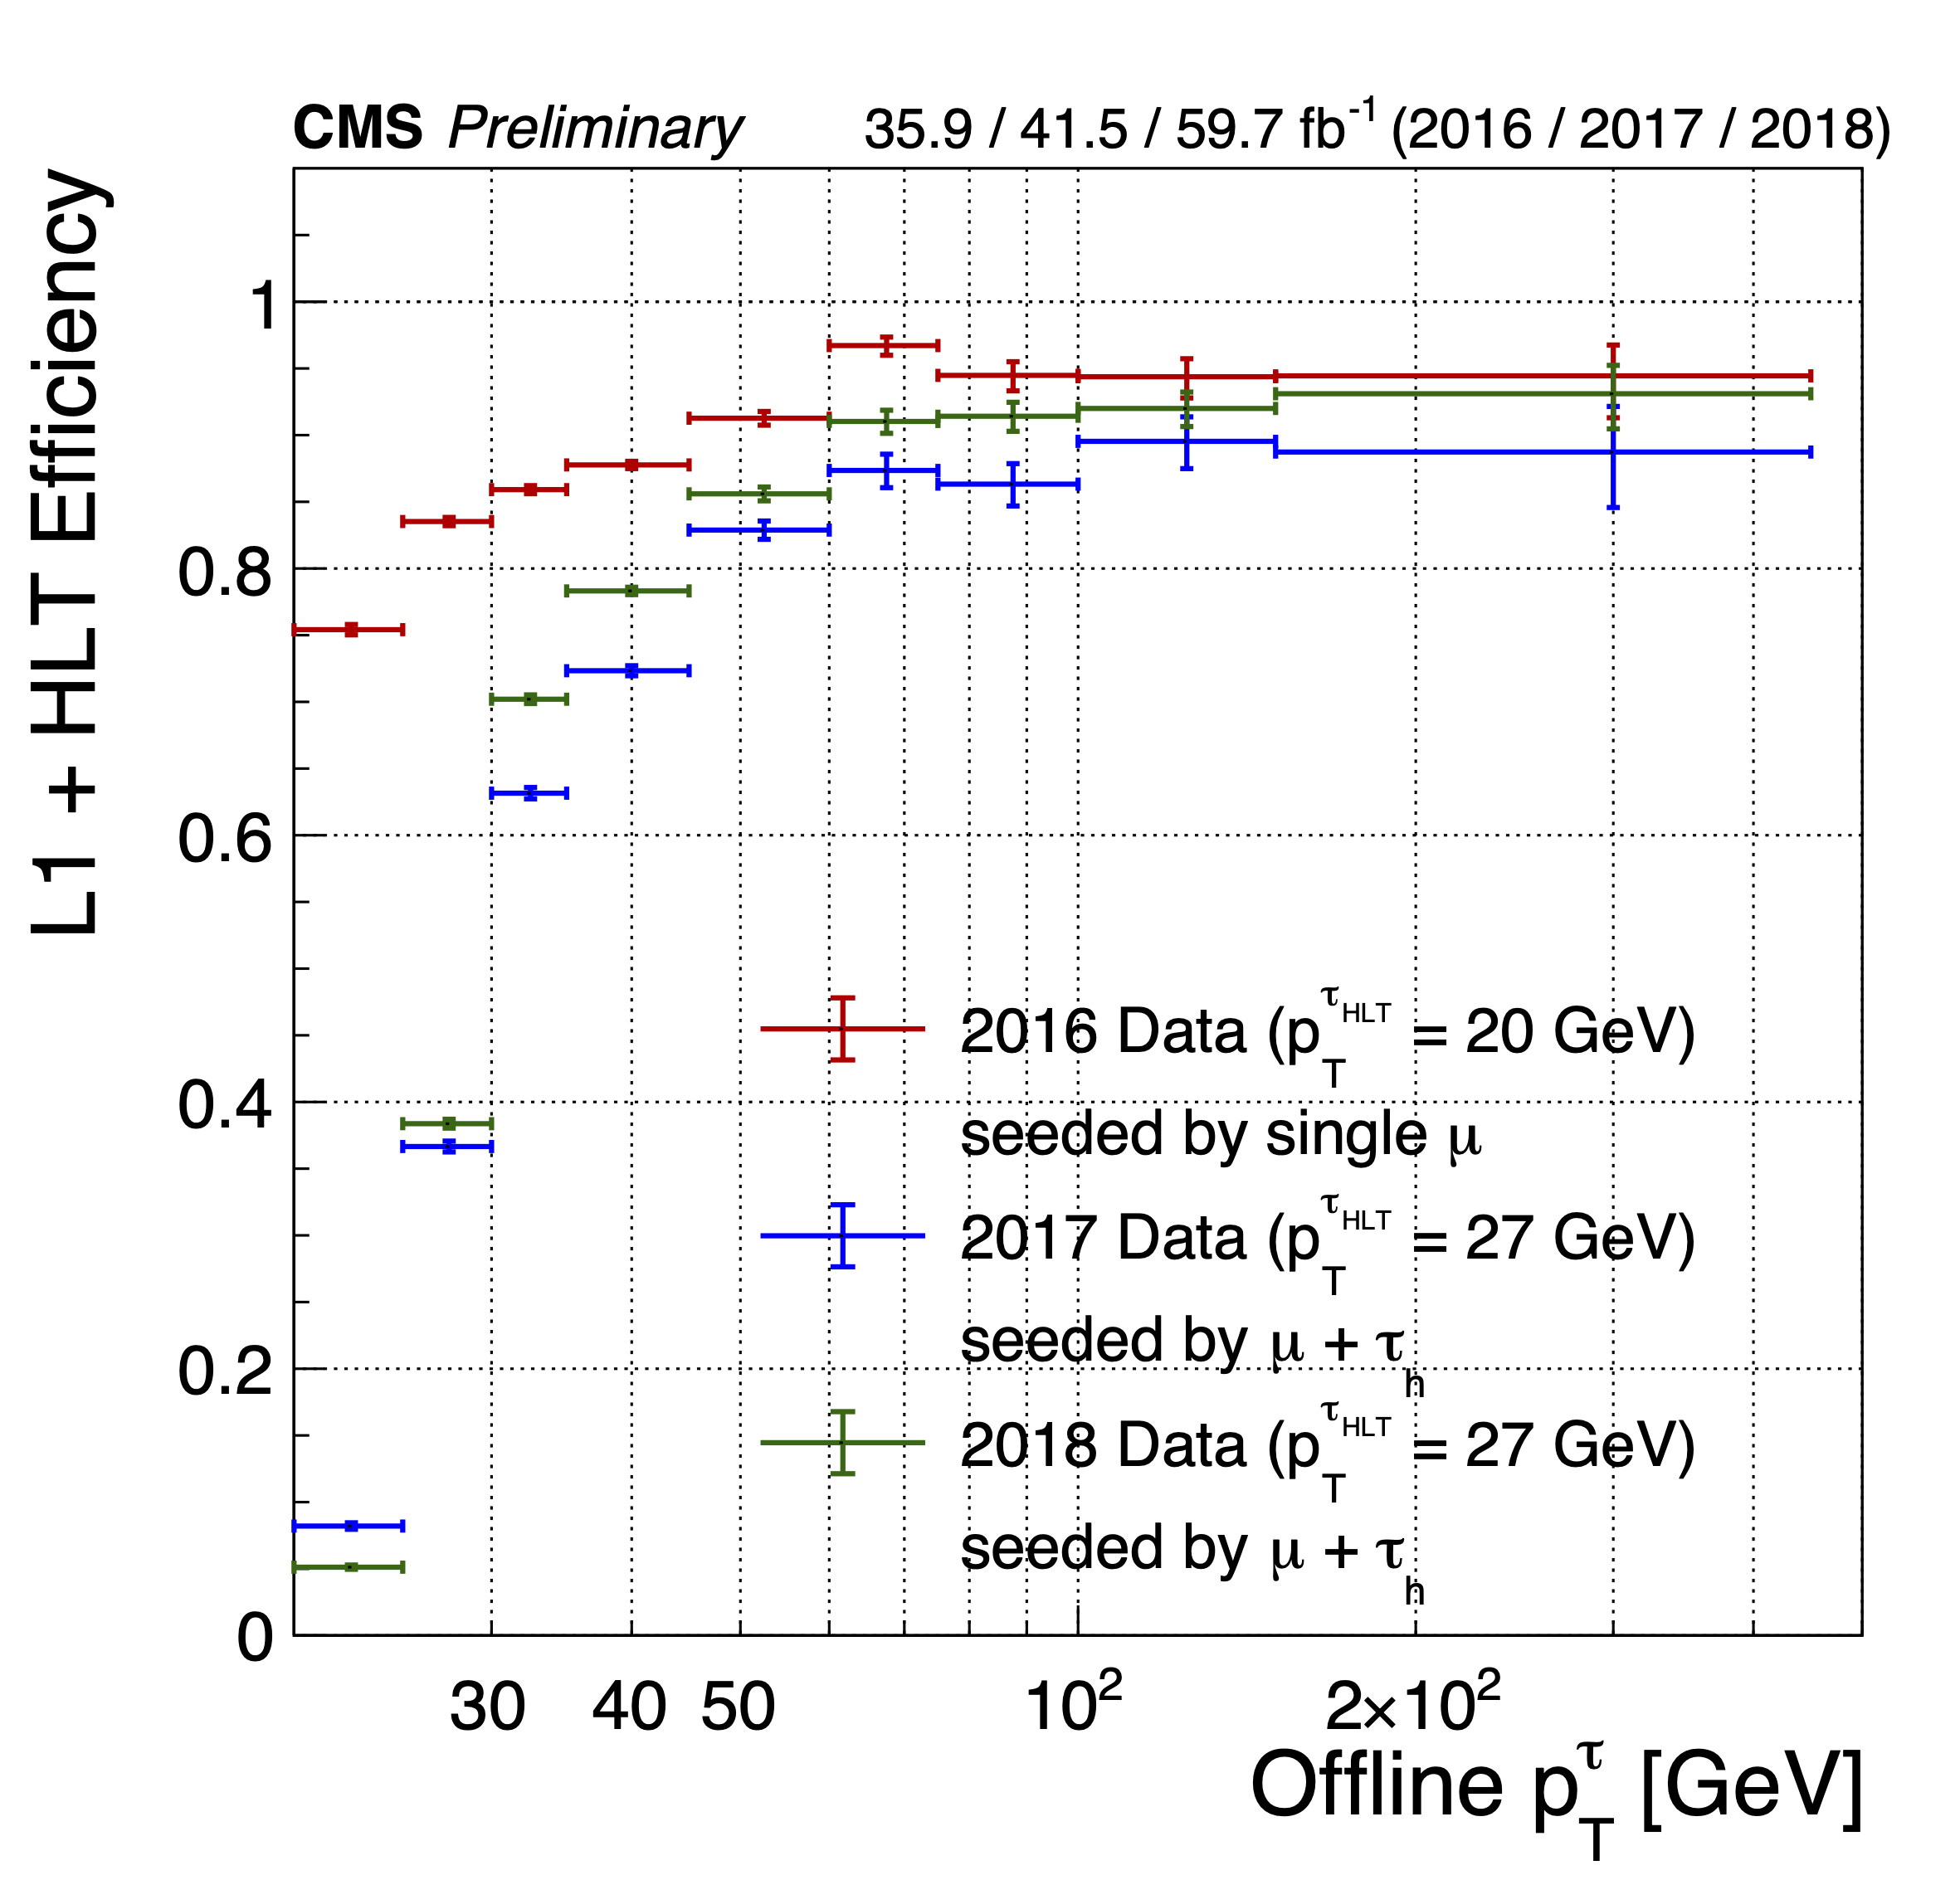
\includegraphics[width=1.0\textwidth]{figures/ch-8-scale-factors-and-corrections/mutauEfficiencyPt_eachYear_mediumTauMVA_Data.png}
        \caption{Mu+tauh cross trigger.}
        \label{fig:mutauEfficiencyPt_eachYear_mediumTauMVA_Data}
    \end{subfigure}
    \hfill
    \begin{subfigure}{0.45\textwidth}
        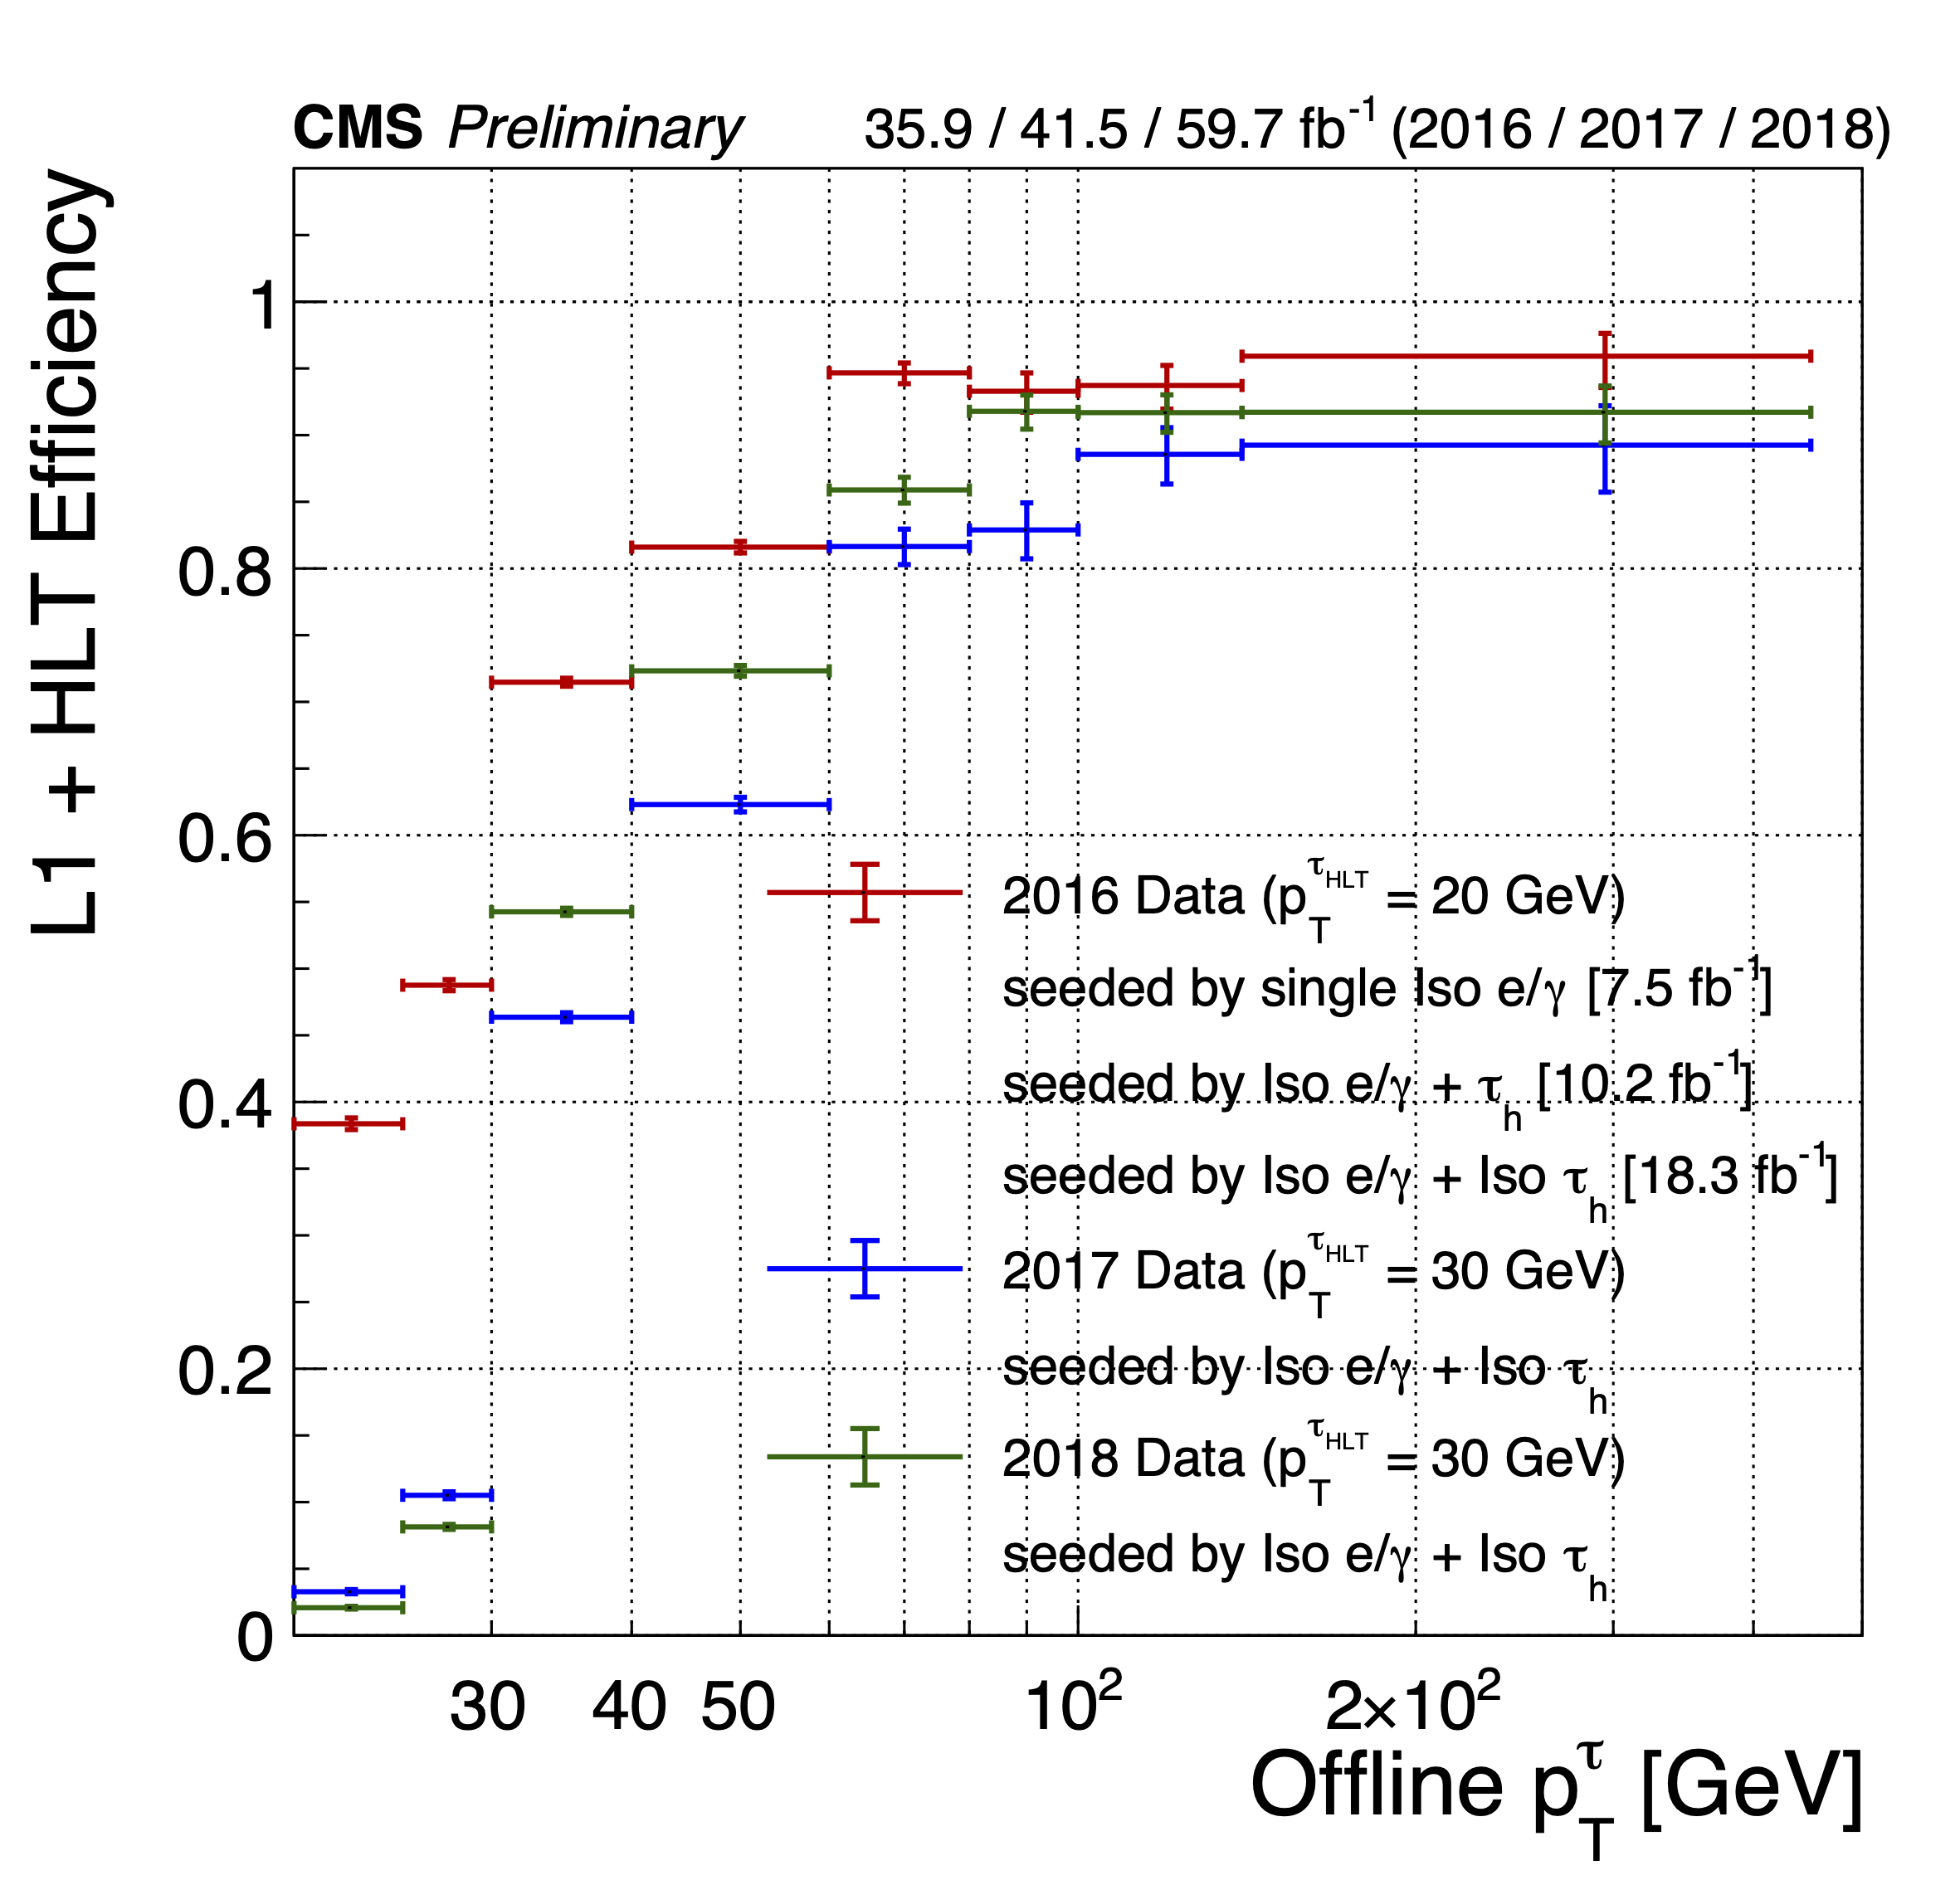
\includegraphics[width=1.0\textwidth]{figures/ch-8-scale-factors-and-corrections/etauEfficiencyPt_eachYear_mediumTauMVA_Data.png}
        \caption{E+tauh cross trigger.}
        \label{fig:etauEfficiencyPt_eachYear_mediumTauMVA_Data}
    \end{subfigure}
    \caption[Hadronic tau leg efficiency of the cross-triggers for $\mu\tau_{h}$ (\textit{left}) and $e\tau_{h}$ (\textit{right}) triggers as a function of offline tau $p_{T}$ for 2016, 2017, and 2018.]{Hadronic tau leg efficiency of the cross-triggers for $\mu\tau_{h}$ (\textit{left}) and $e\tau_{h}$ (\textit{right}) triggers as a function of offline tau $p_{T}$ for the years 2016 (\textit{red}), 2017 (\textit{blue}) and 2018 (\textit{green}), from \cite{twiki_Tau_Lepton_Run_2_trigger_performance}. HLT $p_{T}$ thresholds and L1 seeds are indiated the legends.} 
\end{figure}



\section{Recoil corrections}
\label{sec:ch-8-recoil-corrections}
In proton-proton collisions, W and Z bosons are predominantly produced through quark-antiquark annihilation. Higher-order processes can induce radiated quarks or gluons that recoil against the boson, imparting a non-zero transverse momentum to the boson \cite{2009-Tevatron-recoil-correction}. Recoil corrections accounting for this effect are applied to samples with W+jets, Z+jets, and Higgs bosons \cite{twiki_HiggsToTauTauWorkingLegacyRun2}. The corrections are performed on the vectorial difference between the measured missing transverse momentum and the total transverse momentum of neutrinos originating from the decay of the W, Z, or Higgs boson. This vector is projected onto the axes parallel and orthogonal to the boson $p_{T}$. This vector, and the resulting correction to use, is measured in $Z \rightarrow \mu\mu$ events, since these events have leptonic recoil that do not contain neutrinos, allowing the 4-vector of the Z boson to be be measured precisely. The corrections are binned in generator-level $p_{T}$ of the parent boson and also the number of jets in the event.

\section{Drell-Yan corrections}
The Z boson transverse momentum distribution disagrees between leading-order (LO) simulations and data in a $Z \rightarrow \mu\mu$ control region with at least one b-tag jet \cite{CMS-HIG-17-024}. Per-event weights derived by the 2016 data-only version of this analysis \cite{CMS-HIG-17-024} are applied to $Z \rightarrow \tau\tau / \ell \ell$ events, as a function of the generator-level Z boson $p_{T}$ to provide better matching of MC to data.

\section{Pileup reweighing}
Reweighing is performed to rescale MC events to account for differences between MC and data, in the distribution of the pileup (number of additional proton-proton interactions per bunch crossing). A tool for calculating the pileup reweighing for the MC samples used is provided centrally by the Luminosity POG \cite{twiki_LUMI_POG_recommendation}.

\section{Pre-firing corrections}
TODO: Check 2017 and 2016

\section{Top $p_{T}$ spectrum reweighing}
In Run-1 and Run-2 it was observed that the $p_{T}$ spectra of top quarks in $t\bar{t}$ data was significantly softer than those predicted by MC simulations \cite{twiki_Top_pt_reweighing}. Possible sources of this discrepancy are higher order QCD and/or electroweak corrections, and non-resonant production of $t\bar{t}$-like final states. To account for this, corrections derived from Run-2 data by the Top Physics Analysis Group (PAG) are applied to the $p_{T}$ of the top and anti-top quarks in MC simulations, computed as a function of their generator-level $p_{T}$ \cite{twiki_Top_pt_reweighing}.

\section{B-tagging efficiency}
In order to predict correct b-tagging discriminant distributions and event yields in data, the weight of selected MC events is reweighed according to recommendations by the BTV POG \cite{twiki_btag_SF_methods}. The reweighing depends on the jet $p_{T}$, $\eta$, and the b-tagging discriminant. In this method, there is no migration of events from one b-tag multiplicity bin to another.

\section{Jet energy resolution and jet energy smearing}
Calibration of jet energies, i.e. ensuring that the energy and momentum of the reconstructed jet matches that of the quark/gluon-initiated jet, is a challenging task due to time-dependent changes in the detector response and calibration and high pileup \cite{CMS-JME-13-004} \cite{proceedings-Agarwal:2022txa}. Jet calibration is done via jet energy corrections (JECs) applied to the $p_{T}$ of jets in MC samples, accounting successively for the effects of pileup, uniformity of the detector response, and residual data-simulation jet energy scale differences \cite{twiki_JetResolution_JEC}. Typical jet energy resolutions reported at $\sqrt{s} = 8$ TeV in the central rapidities are 15-20\% at 30 GeV and about 10\% at 100 GeV \cite{CMS-JME-13-004}. Jet energy corrections are also propagated to the missing transverse energy.

Measurements show that the jet energy resolution (JER) in data is worse than in simulation, and so the jets in MC need to be smeared to describe the data. JER corrections are applied after JEC on MC simulations, and adjust the width of the $p_{T}$ distribution based on pileup, jet size, and jet flavour \cite{twiki_JetResolution_JER}. Tools for applying JEC and JER are provided centrally by the JER Corrections group. 